\subsection{Mass Budget }
The mass estimate for HurriSat is based on previous successful 6U cubesat missions and commercial data sheet for sub-components weights \cite{Cipera2018}. Typically a 6U CubeSat is 20 cm × 10 cm × 34.05 cm. After listing every single component in the payload, the total weight is determined by summing them all at once. Then the rest of subsystem sections are determined based on percentage values from reference sheets \cite{NASA2018}.  Table \ref{Tab:ms} shows the mass sizing based on the total payload mass. Payload is estimated to be approximately 3.1kg after sizing. This includes dual high-tech cameras, LiDAR, IC electronics, and censors outlined in the payload section.

\subsection{Power Budget }
\caption{Power Budget}
The power budget placed on each subsystem is shown in Table \ref{Tab:ps} and a 30\% margin is taken into account. This specif values are obtained based on the components the payload houses first. Each component's power is summed up and determined before to estimate the total payload power consummation. It's from then that each of subsystem's power are determined. \\

\begin{table}[hbt!]
\parbox{.5\linewidth}{
\centering
                \begin{tabular}{ll}
                    
                        \rowcolor{gray!50} 
                        \textbf{Element}       & \textbf{Power (W)} \\ \hline
                        Payload       & 5.8                \\
                        ADCS          & 8                  \\
                        C\&DH         & 1                  \\
                        Power         & 9                  \\
                        Propulsion    & 12                 \\
                        Structure     & 0                  \\
                        Thermal      & 0                  \\
                        Communication & 1                  \\
                        Margin        & 30\%               \\ \hline
                        Total         & 47.84 \\
                \end{tabular}
                    \caption{Power Sizing}
                    \label{Tab:ps}
        }
\hfill
\parbox{.5\linewidth}{
\centering
                \begin{tabular}{ll}
                        \rowcolor{gray!50}
                        \textbf{Subsystem}      & \textbf{Mass (kg)} \\ \hline
                        Payload     & 0.172 \\ 
                        ADCS        & 0.284 \\  
                        C\&D        & 0.13 \\
                        Power       & 1.283 \\  
                        Propulsion  & 3.49 \\  
                        Structure   & 1.2 \\
                        Thermal     & 1.757 \\
                        Margin      & 10\% \\\hline
                        Total       & 7.2325 \\
                \end{tabular}
\caption{Mass Sizing}
\label{Tab:ms}
}
\end{table}
\vspace{1cm}
\subsection{$\Delta{V_{design}}$ Budget }
The delta-v budget is an estimate of the total change in velocity required for the space mission. It is calculated as the sum of the delta-v required to perform each propulsive maneuver needed during the mission. It also determines the propellant is required for HurriSat at a given given empty mass and propulsion system. The Delta V design required for the spacecraft was observed over a range of possible altitudes and inclination angles. The range was selected after a thorough research of LEO Cubesats (see Figure \ref{fig:graph} for more trade studies) that operate on the the optimum orbit. Table \ref{Tab:dv} shows the values with the best parameters listed. The intersection cell (highlighted cell in bright red) is our optimum $\Delta v_{design}=11.729km/s$. Selected choice of altitude is $h=800km$, and the inclination angle is $\alpha = 35$. \\

\begin{table}[hbt!]
\centering 
\caption{$\Delta{V_{design}}$ in (km/s)}
% \resizebox{\textwidth}{!}{%
\begin{tabular}{ccccccc}
\multicolumn{1}{c}{\rowcolor{gray!50}Altitude (km)} & \multicolumn{6}{c}{\rowcolor{gray!50}Inclination Angle \alpha (degrees)} \\
\hline                                  & 30    & 32    & \cellcolor{red!20}35    & 40    & 45    & 52    \\
\rowcolor{red!20} 800   & 11.709 & 11.717 & \cellcolor{red!40}11.729 & 11.752 & 11.778 & 11.817 \\
850                               & 11.836 & 11.843 & \cellcolor{red!20}11.856 & 11.879 & 11.904 & 11.943 \\
900                               & 11.958 & 11.966 & \cellcolor{red!20}11.978 & 12.001 & 12.026 & 12.065 \\
950                               & 12.077 & 12.084 & \cellcolor{red!20}12.097 & 12.119 & 12.144 & 12.183 \\
1000                              & 12.191 & 12.199 & \cellcolor{red!20}12.211 & 12.234 & 12.258 & 12.297 \\
1100                              & 12.410 & 12.418 & \cellcolor{red!20}12.430 & 12.452 & 12.476 & 12.514 \\
1200                              & 12.617 & 12.624 & \cellcolor{red!20}12.636 & 12.658 & 12.682 & 12.720
\end{tabular}
\label{Tab:dv}
\end{table}

\subsection{Cost Budget}

Cost budget is a financial plan exhibiting the expected costs related to running a business or undertaking a project or for developing a product. Cost budget are prepared for those expenses which are significant for the project. The maximum cost budget for CSLI missions is capped at $300,000USD$ by NASA. It's still difficult to accurately provide the cost for HurriSat. This is mostly because the technology and commercialization of these satellites is still in its infancy stages. Based on the findings from Space Flight \cite{SpaceFlight} HurriSat is estimated to cost around $48-50k$ USD per unit excluding labor costs. Every other component cost is listed in Figure \ref{fig:cost}. The stake holders should know that cost is driven by supply and demand, and thus a steeper price change is expected given the manufacturing challenges.\\
\vspace{1cm}
\FloatBarrier
\begin{figure}[hbt!]
    \centering
    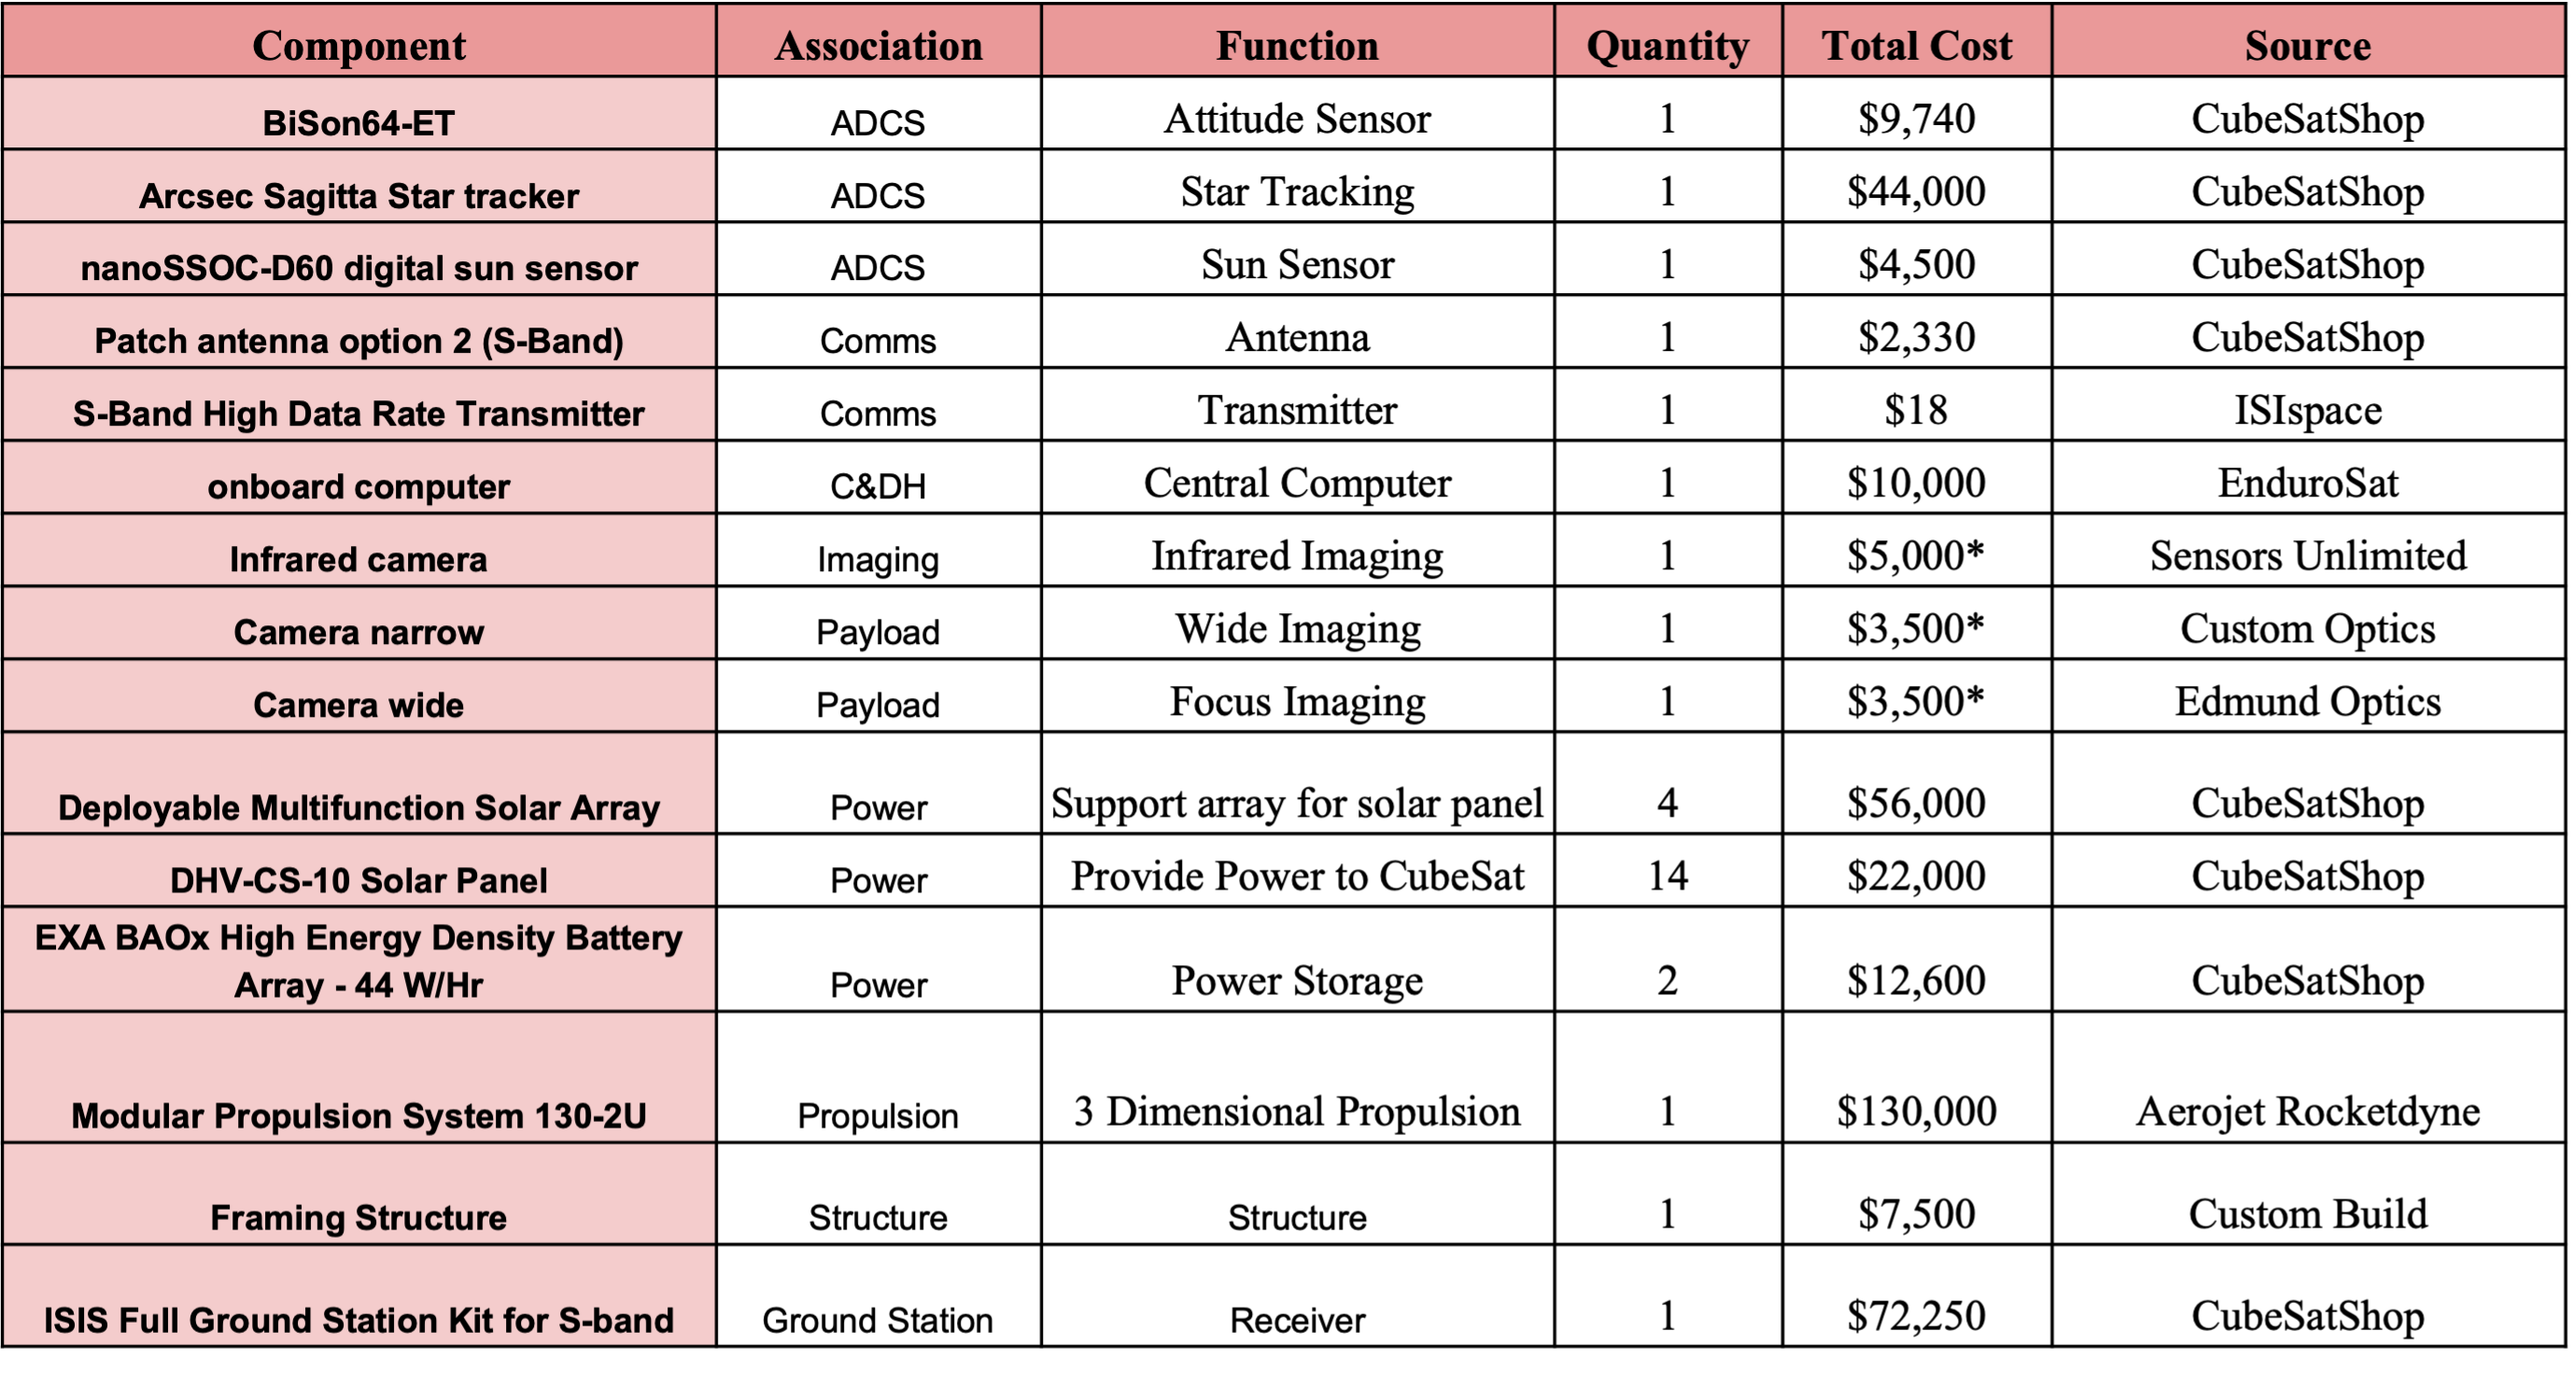
\includegraphics[width=\textwidth, frame]{Images/cost.png}
    \caption{Cost Budget}
    \label{fig:cost}
\end{figure}

\vspace{1cm}

Based on previous research done at PRICE, it's obvious planetary missions tend to cost more than similar ones that stay near the Earth. NASA’s attempt at a planetary CubeSat demonstrates that these unique satellites are becoming a permanent part of space exploration. The sum of each component listed in the figure comes to about $251,000USD$ cost. There are still installation, maintencae and testing overheads to account for. But those can only be estimated once the manufacturing phase starts. \\

\newpage
\subsection{Cubesat Sizing}
HurriSat's sizing is represented in Figure \ref{fig:hurrisat} down below. The main components are laid out, and labeled. Note that actual sized may vary upon manufacturing and delivery. But the figure is to show how the components are aligned in a manner that's able to fit the cubesat's purpose whilst keeping it's axis of symmetry intact. The subsystem components are shown as boxed figures for place holding. ALl these components are estimated from the dimensions provided in the commercial manufacturing data sheet. It should be  noted that the main frame casing is custom built with Aluminum Alloy. The number of solar panels and solar cells are designed in such a way to reflect the values proposed as per the power budget. \\[.2in]

\begin{figure}[hbt!]
    \centering
    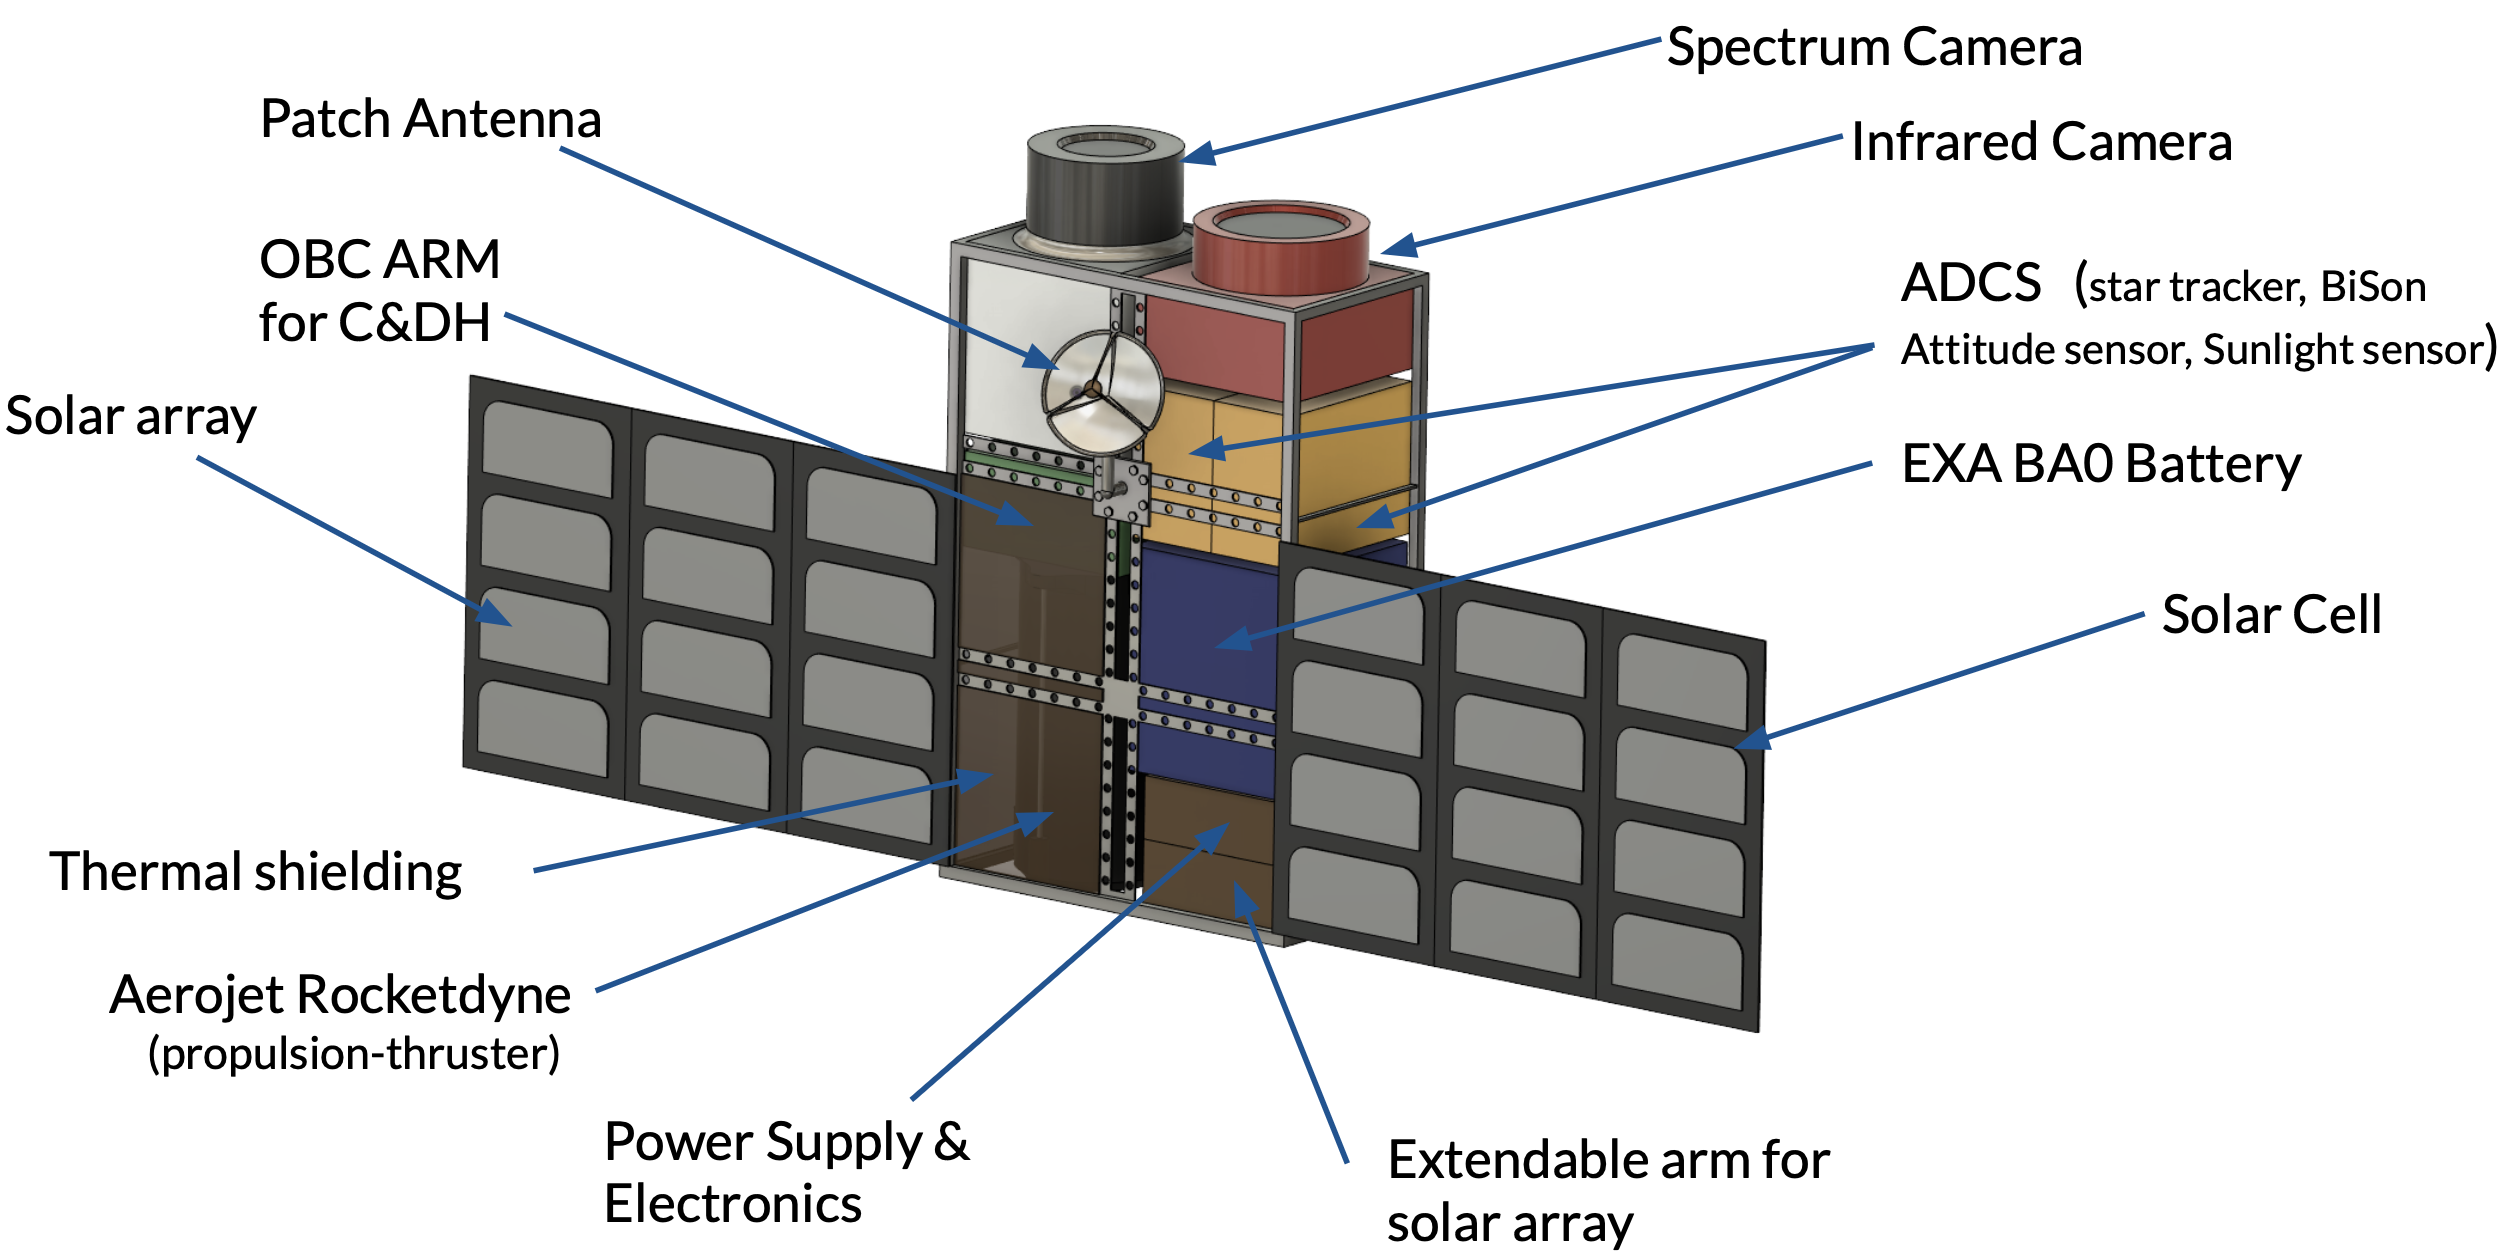
\includegraphics[width=\textwidth,frame, keepaspectratio]{Images/hurrisat.png}
    \caption{HurriSat and its Components}
    \label{fig:hurrisat}
\end{figure}
\vspace{0.5cm}
\subsection{Cubesat Configuration}
HurriSat is designed to easily accommodate in the launch launch vehicle. In Figure \ref{fig:folded} it is fully closed  for transportation and the Falcon 9 launching phase.  This easy packaging  helps minimize collision impact and prevent any launch associated risks, like mechanical, vibrational, electrical or acoustic energy.  The Semi folded \ref{fig:iso} shows how the solar arrays for cubesat extend during the transition from parking to operational orbit inorder to gain some solar power. This sets up the satellite ready for operation. Mechanical lever arms are utilized to push the folded panels away from the unit without any hydraulic system. Figure \ref{fig:stretch} is a fully extended HurriSat during and on operation at the desired orbit. Cold thrustures can be used to maneuver the cubesat with the aid of the ADSC and thrusters at hand.
\begin{figure}
    \centering
    \subfloat[Clothed and Intact]{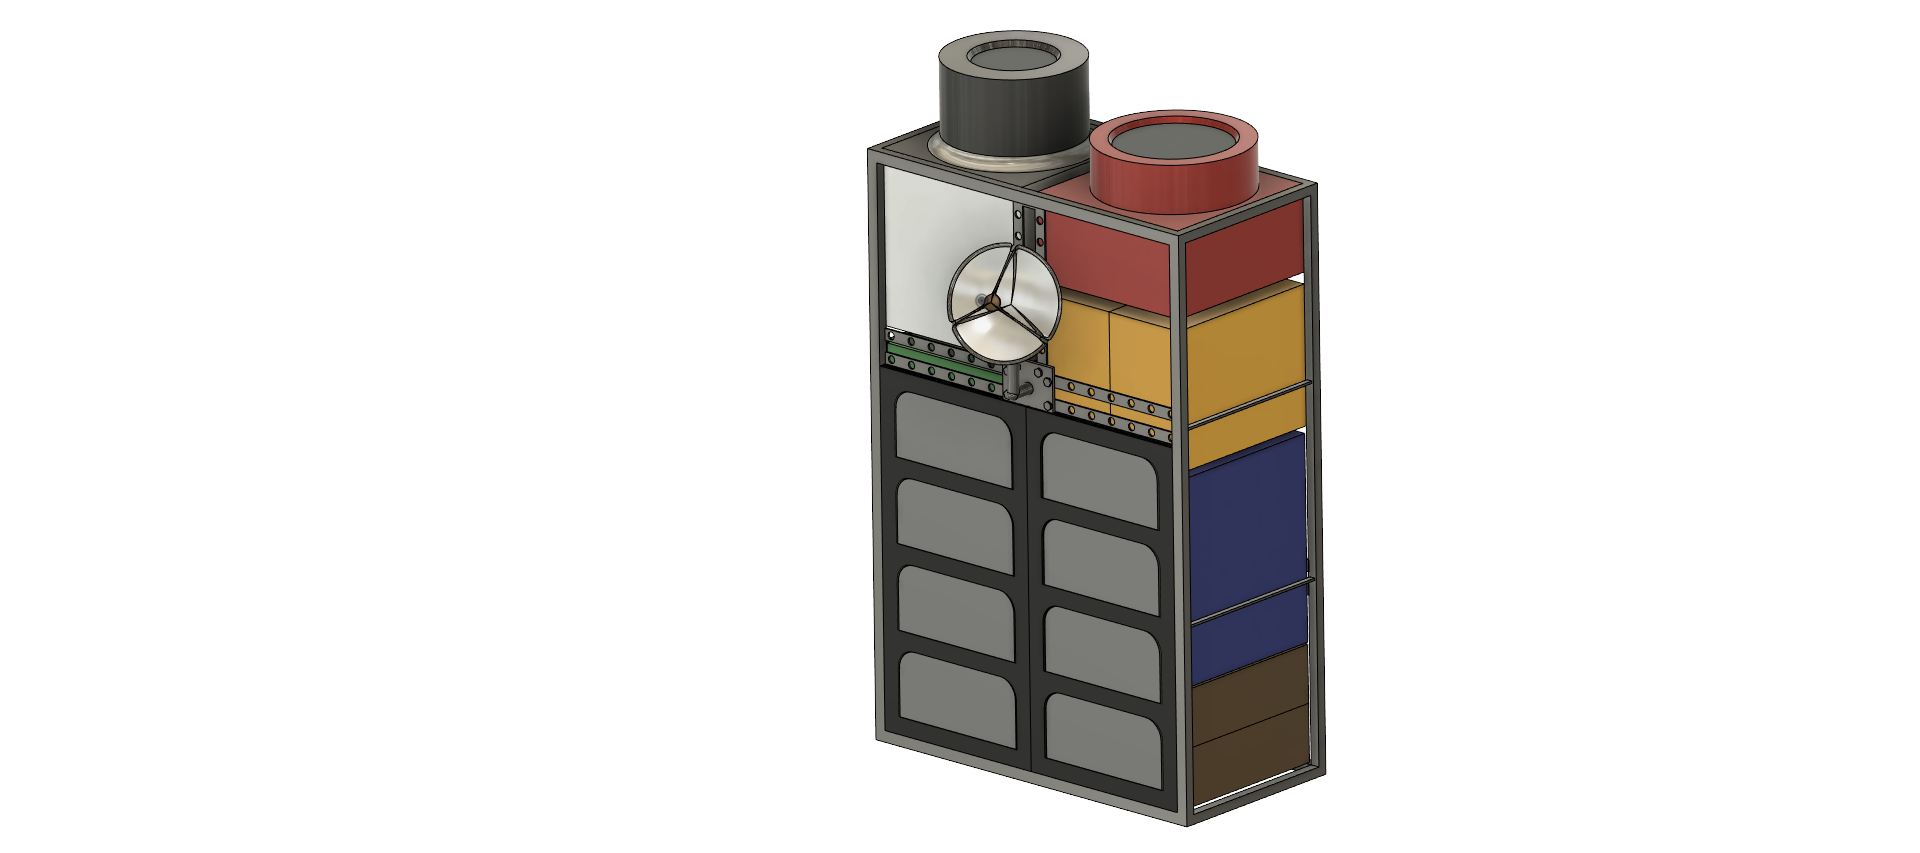
\includegraphics[width=0.8\textwidth,scale=0.6]{Images/folded.png}\label{fig:folded}}\\[.2in]
    \subfloat[Unfolding Phase]{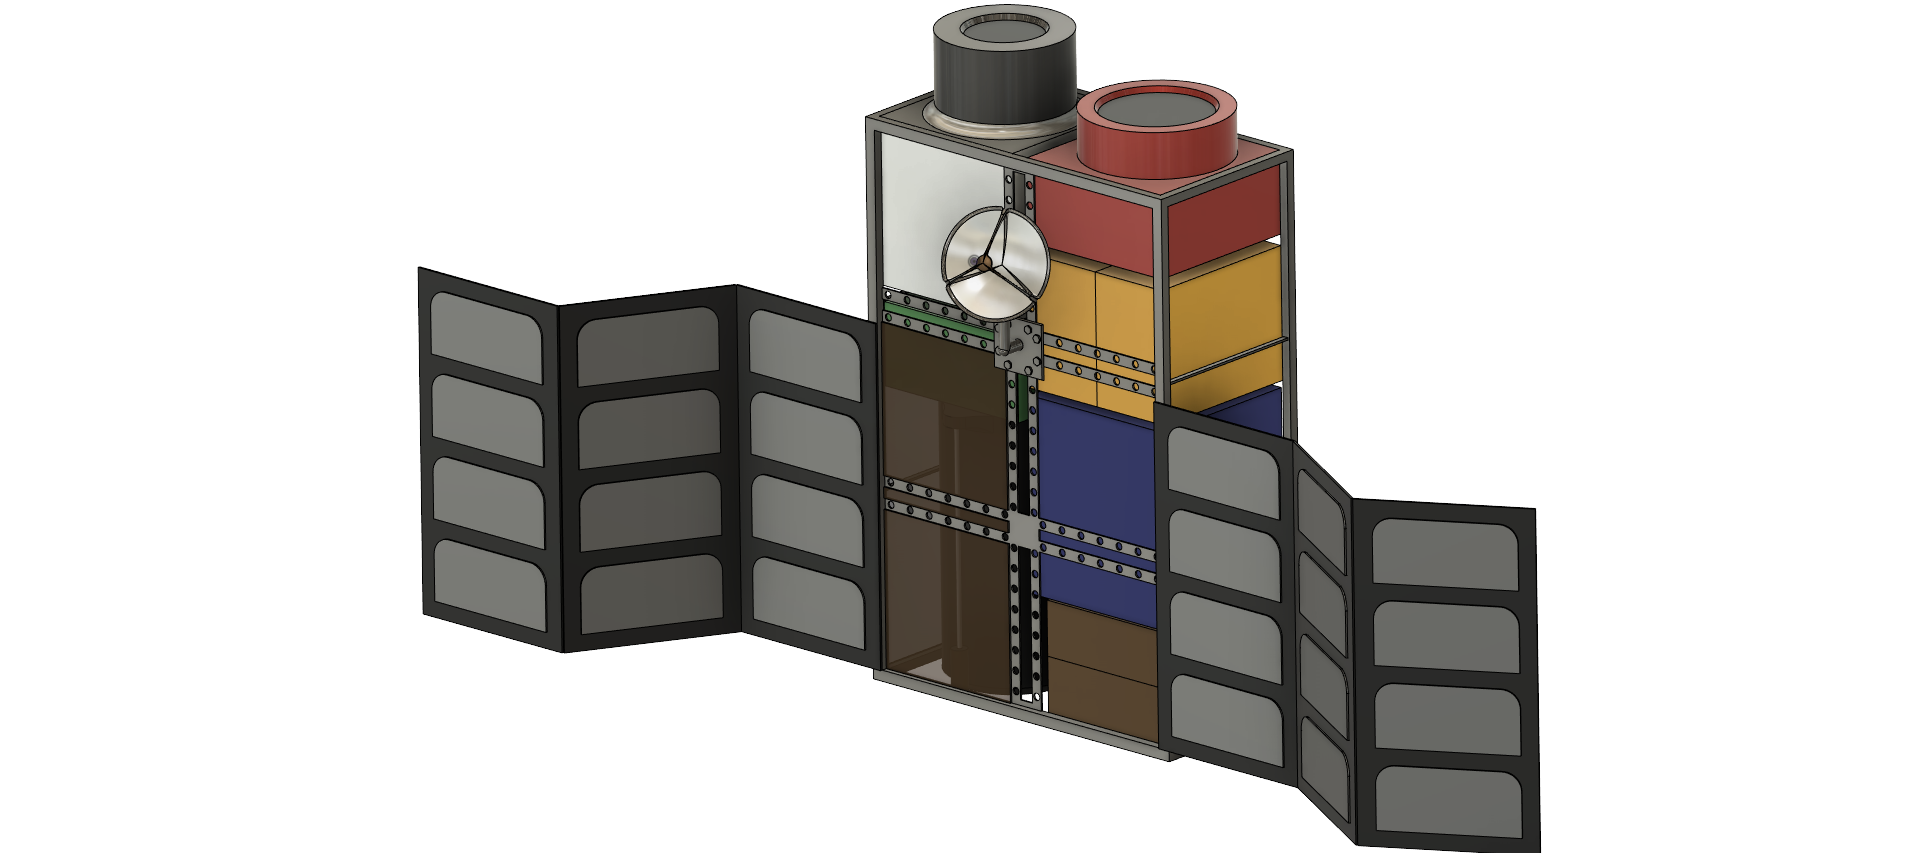
\includegraphics[width=0.9\textwidth, scale=0.8]{Images/iso.png}\label{fig:iso}}
    \qquad
    \subfloat[Fully Stretched]{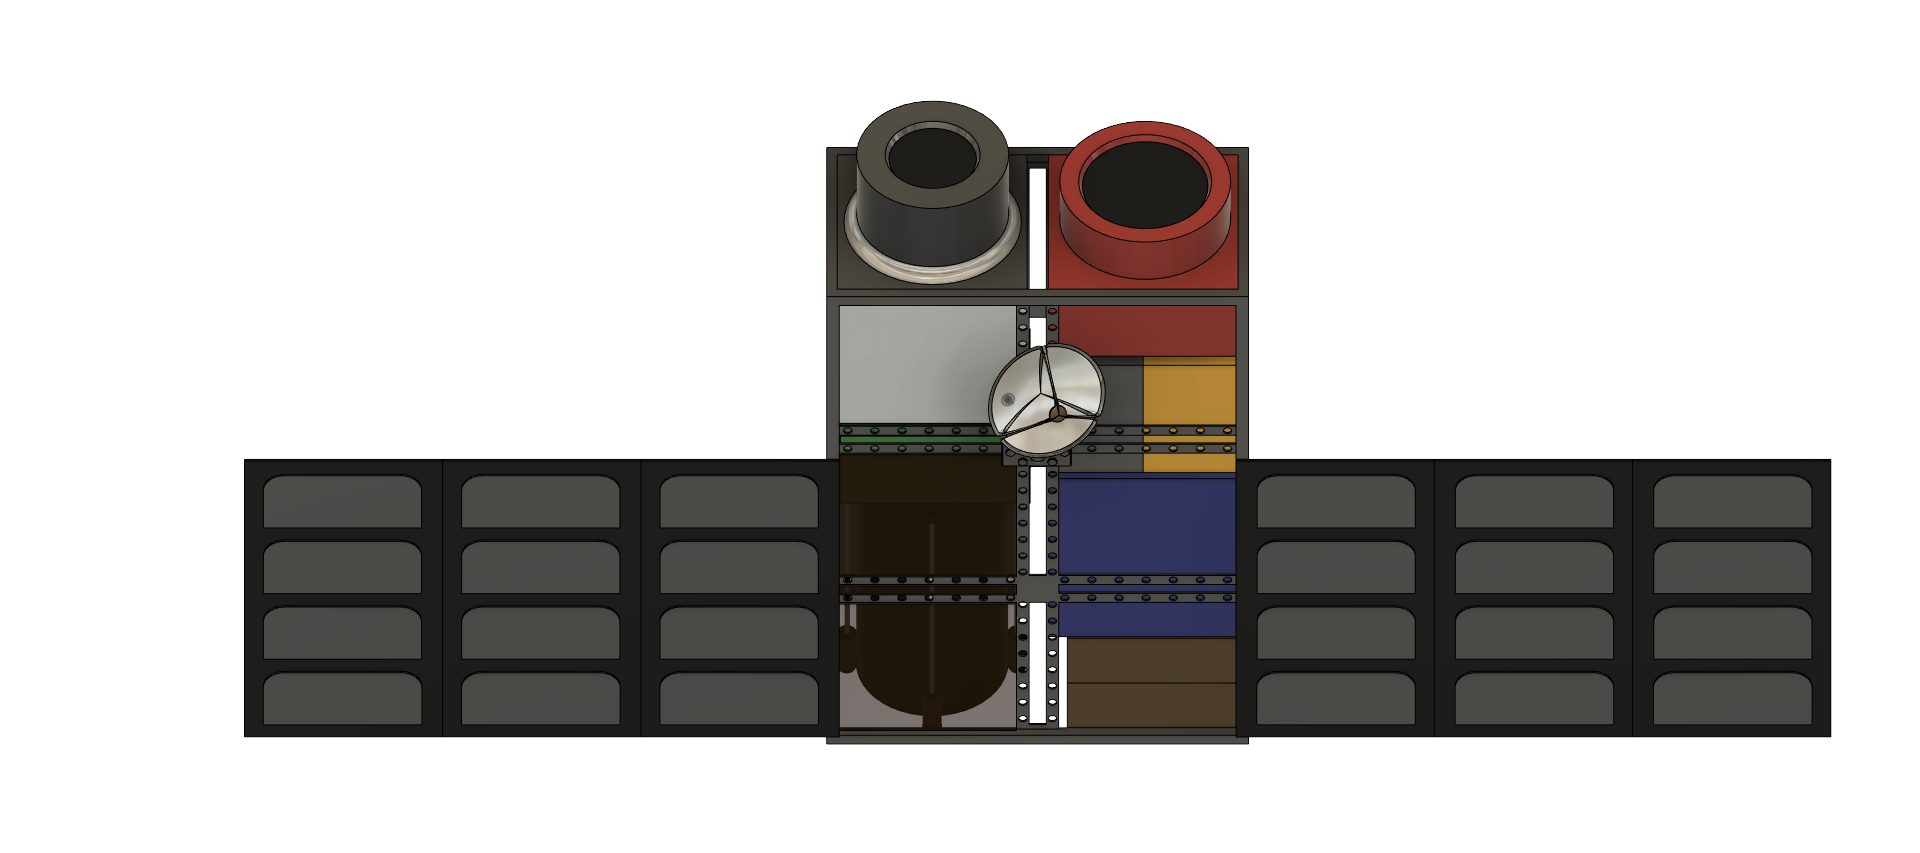
\includegraphics[width=0.8\textwidth,scale=0.9]{Images/stretch2.png}\label{fig:stretch}}
    \caption{HurriSat Launch Configuration}
    \label{fig:config}
\end{figure}